\documentclass[../main.tex]{subfiles}
\begin{document}
\chapter{FedRAMP - Federal Risk and Authorization Management Program}
\section{Introduzione}
In questo capitolo verrà approfondito FedRAMP, il programma federale americano per la gestione del rischio e delle autorizzazioni nella cloud.
Sarà proposta un'analisi degli obiettivi del programma, specificando le problematiche in esso affrontate in relazione anche a quanto descritto nel capitolo precedente.
Verrà poi esposta la struttura del documento, dopodiché ci si concentrerà sulla struttura dello stesso approfondendo i ruoli degli attori coinvolti.
In conclusione saranno esposti i concetti di \textit{readiness} e di \textit{compliance} al programma, e sarà approfondito il ruolo dello stesso in Amazon AWS.

\section{Cos'è FedRAMP}
FedRAMP è il programma governativo americano l'applicazione del \textbf{FISMA} (Federal Information Security Management Act) nell'adozione di tecnologie cloud.
Esso propone un approccio standardizzato al \textit{security assessment}, alle autorizzazioni e al monitoraggio continuo di prodotti e servizi cloud, fornendo un insieme di requisiti di sicurezza e un programma di assessment indipendente, nato dalla collaborazione di esperti di sicurezza e di tecnologie cloud.
Le entità coinvolte nella redazione di questo programma sono state molte: la General Services Administration (GSA), il National Institute of Standards and Technology (NIST), il dipartimento di Sicurezza Nazionale (Department of Homeland Security, DHS), il dipartimento della Difesa (Department of Defense, DOD), la National Security Agency (NSA), l'Office of Management and Budget (OMB).

I \textit{cloud service provider} che vogliono offrire servizi per la pubblica amministrazione americana e gli uffici federali devono essere autorizzati tramite questo programma.
Nonostante sia stato sviluppato nel contesto USA, la dinamicità e l'elasticità di FedRAMP ne ha permesso l'adozione \textit{de-facto} anche in altre nazioni, specialmente dell'Asia orientale e del nord Europa.
\subsection{FISMA, Federal Information Security Management Act}
Il FISMA è uno standard di sicurezza, entrato in vigore come legge il 17 Dicembre 2002 come "Titolo III" dell'E-Government Act\cite{united2004information}.
Esso definisce tre obiettivi principali per la sicurezza dei sistemi informativi federali:
\begin{itemize}
    \item \textbf{Confidenzialità}, per garantire restrizioni autorizzate sull'accesso e la \textit{disclosure} dei dati, con l'obiettivo di proteggere la privacy ed eventuale informazioni sul proprietario odegli stessi
    \item \textbf{Integrità}, per proteggere il dato da manipolazioni o azioni distruttive e per garantire allo stesso tempo l'autenticità e la non-repudiabilità dell'informazione
    \item \textbf{Disponibilità}, per assicurare condizioni di affidabilità nell'accesso al dato
\end{itemize}

A tal fine il \textbf{NIST} ha prodotto il \textbf{Federal Information Risk Management Framework}(\textit{RMF}) il quale organizza i sistemi informatici sulla base del livello di rischio (basso, medio alto) e descrive un insieme minimo di requisiti che devono essere rispettati per garantire un livello di sicurezza adeguato\cite{nist2003nist}.

\begin{figure}[H]
\centering
\makebox[\textwidth]{
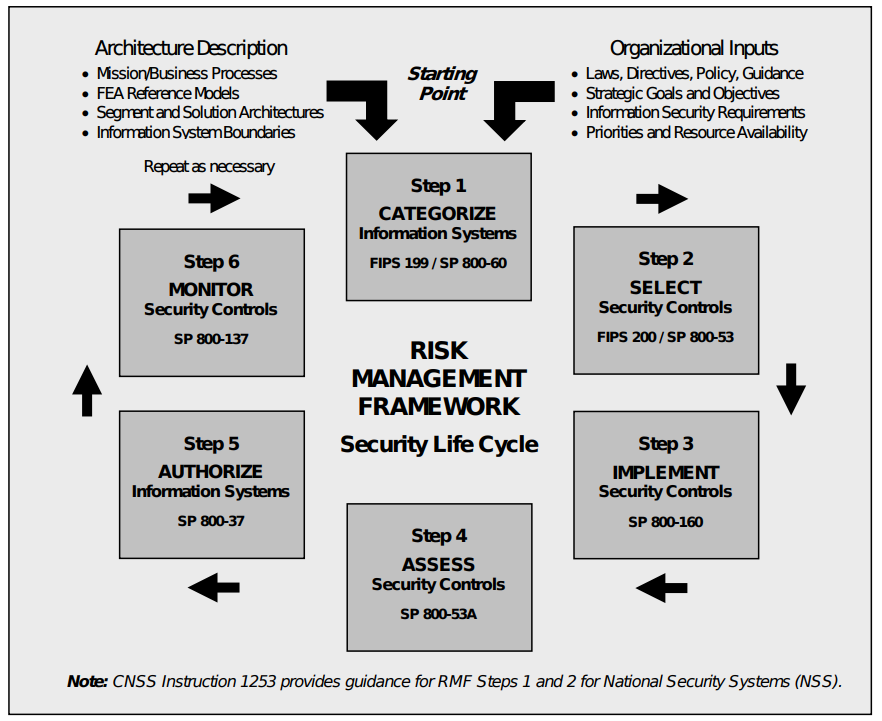
\includegraphics[width=\textwidth]{immagini/risk_management_framework.png}
}
\caption{Risk Management Framework, da \cite{nist2003nist} }\label{fig:riskmanagementfw}
\end{figure}

Tramite la figura \ref{fig:riskmanagementfw} è possibile identificare le sei fasi che compongono il processo di gestione del rischio identificato dal framework.
Tramite i documenti FIPS 199 e NIST SP 800-60 è possibile effettuare la categorizzazione dei sistemi informativi, successivamente si può procedere con la selezione dei controlli di sicurezza mediante FIPS 200 e SP 800-53. La fase successiva è quella implementativa, regolata dal documento SP 800-160, seguita dall'assessment dei controlli di sicurezza (SP 800-53A); successivamente si può procedere con l'autorizzazione del sistema informativo (SP 800-37) e con la fase di monitoraggio.
Il processo di gestione del rischio illustrato è quindi ciclico e continuo.


\section{Struttura}
.\\\newpage
.\\\newpage
.\\\newpage
.\\\newpage
\section{FedRAMP readiness}
.\\\newpage
.\\\newpage
.\\\newpage
.\\\newpage
\section{Controlli di sicurezza per la conformità}
.\\\newpage
.\\\newpage
.\\\newpage
.\\\newpage
\section{FedRAMP in Amazon AWS}
.\\\newpage
.\\\newpage
\end{document}
